\section{Results}
\label{sec:results}

\subsection{Reliability and provenance across heterogeneous infrastructure}
\label{sec:reliability-results}

We report the per-origin behavior breakdown, retained model autonomy, and contract-violation counts for the same eight real runs used in Section~\ref{sec:b2-confound}: common-denominator (CD) and corrected platform-tuned (PT) configurations, both workloads, both systems, real concurrent load, at the most solid available repetition count for each combination. The ``invalid after repair'' figure reflects a proposal's validity after the pipeline's own repair-retry budget is exhausted, not the model's raw first-pass output, so it measures how often repair alone fails to recover a usable structured output rather than raw generation quality.

\begin{table}[t]
\centering
\footnotesize
\caption{Reliability and provenance profile of the eight real runs underlying Section~\ref{sec:b2-confound} (System A: AMD; System B: NVIDIA. Mode CD: common-denominator; PT: platform-tuned, corrected configuration). All rates are shares of committed steps; lower is better for ``invalid after repair'' and for violations, higher is better for ``semantic-valid'' and ``autonomy rate.'' Violations are reported as (must-not~/~bounded~/~cardinality~/~state-mutation) counts, not rates, since they are rare events (4 total across all 46{,}701 steps).}
\label{tab:reliability}
\resizebox{\textwidth}{!}{%
\begin{tabular}{llcrrrrrrl}
\toprule
System & Workload & Mode & Steps & \shortstack{Invalid\\after repair} & \shortstack{Repair\\attempted} & \shortstack{Semantic-\\valid} & \shortstack{Guard-added\\msgs/step} & \shortstack{Guard-added\\actions/step} & \shortstack{Autonomy\\rate} \\
\midrule
A (AMD) & disaster-response & CD & 11{,}655 & 64.8\% & 82.1\% & 35.2\% & 1.11 & 0.26 & 0.02\% \\
A (AMD) & disaster-response & PT & 11{,}663 & 65.2\% & 81.5\% & 34.8\% & 1.11 & 0.26 & 0.01\% \\
A (AMD) & supply-chain       & CD & 4{,}393  & 59.8\% & 75.8\% & 40.2\% & 1.47 & 0.017 & 0.00\% \\
A (AMD) & supply-chain       & PT & 4{,}395  & 59.9\% & 74.0\% & 40.1\% & 1.47 & 0.017 & 0.00\% \\
B (NVIDIA) & disaster-response & CD & 5{,}832 & 48.9\% & 58.6\% & 51.1\% & 1.11 & 0.26 & 0.00\% \\
B (NVIDIA) & disaster-response & PT & 5{,}835 & 47.4\% & 57.8\% & 52.6\% & 1.11 & 0.26 & 0.00\% \\
B (NVIDIA) & supply-chain       & CD & 1{,}464 & 56.6\% & 63.7\% & 43.4\% & 1.48 & 0.016 & 0.00\% \\
B (NVIDIA) & supply-chain       & PT & 1{,}464 & 58.5\% & 64.3\% & 41.5\% & 1.48 & 0.016 & 0.00\% \\
\bottomrule
\end{tabular}%
}
\end{table}

Three findings follow, in order of importance.

First, and most consequential for RQ3, retained model autonomy is effectively zero across every system, workload, and configuration (0.00--0.02\%, indistinguishable from zero at this precision). A real 7--8B instruct model produces genuinely variable free-text completions, yet essentially none of the runtime's committed messages or actions in this dataset trace back to a raw, unmodified model proposal: the policy-completion layer supplies the committed behavior in practically every step. Useful-step coverage is nonetheless 99.99\% (11{,}654 of 11{,}655 steps on the largest run). The simulation keeps producing contract-satisfying, committed behavior throughout, but that reliability is achieved by the scaffolding around the model, not by the model. This is precisely the distinction RQ3 asks a runtime to make explicit, and precisely where contracts can conceal a loss of model agency if the two figures are not reported side by side.

Second, raw model output is invalid, even after in-loop repair, roughly half the time (47--65\% across combinations), with repair attempted on 58--82\% of steps. Repair attempts and final invalidity move together rather than inversely: attempting repair more often does not correspond to a lower final-invalid rate across these rows. The repair loop's fixed retry budget appears to recover a minority of malformed completions rather than reliably rescue them, and policy completion, not repair, is what keeps useful-step coverage near 100\%.

Third, the two configuration modes are nearly identical on every reliability metric within a system/workload pair (for example, System A disaster-response invalid rate 64.8\% versus 65.2\%; System B disaster-response semantic-valid 51.1\% versus 52.6\%), visible directly in Table~\ref{tab:reliability} and Figure~\ref{fig:reliability}. This is expected and serves as an internal check, since the two configurations differ only in serving parameters (batching and concurrency limits, with precision already fixed identically), never in model weights or scenario logic. Reliability behavior should, and does, stay stable across the throughput reversal reported in Section~\ref{sec:b2-confound}. Contract violations are rare on both systems, 4 total across 46{,}701 combined steps (3 state-mutation and 1 must-not, all on System A), and we report them exactly as observed rather than round them to zero.

\begin{figure}[t]
\centering
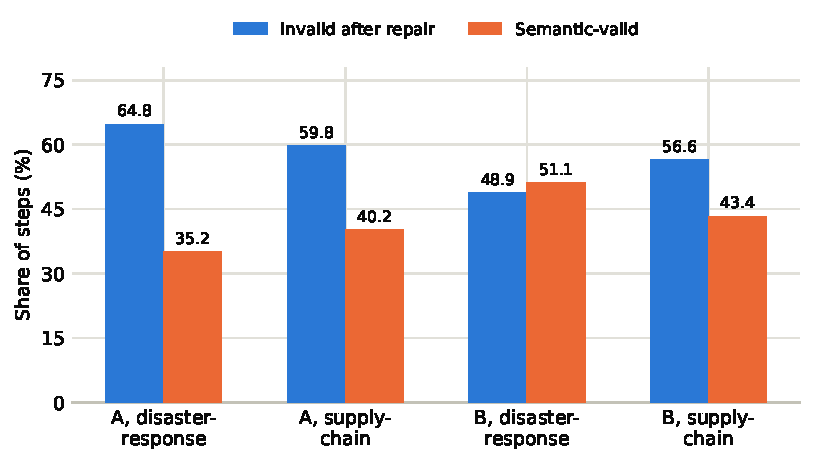
\includegraphics[width=0.82\textwidth]{figures/fig_reliability.pdf}
\caption{Invalid-after-repair rate and semantic-valid rate by system and workload, common-denominator configuration (platform-tuned values omitted: Section~\ref{sec:reliability-results} shows they are nearly identical; the full eight-row breakdown is in Table~\ref{tab:reliability}). Bars show the share of committed steps; higher is better for semantic-valid, lower is better for invalid-after-repair.}
\label{fig:reliability}
\end{figure}

One cross-system pattern is worth flagging cautiously rather than over-interpreting. System B's invalid-output rate is consistently lower than System A's on the disaster-response workload (approximately 48\% versus 65\%) despite an identical model revision, identical numeric precision for cached attention state, and near-identical decoding parameters. Per Section~\ref{sec:non-claims}, we do not claim this isolates an accelerator-vendor effect: the two systems also differ by one minor release of the serving software and in the underlying attention-kernel implementation actually exercised, either of which could plausibly explain a generation-quality difference of this size. We treat this as the kind of software-maturity confound discussed in Section~\ref{sec:limitations}, an open observation rather than a resolved hardware claim.

\subsection[Platform-tuned vs.\ common-denominator: a confound, found and corrected]{Platform-tuned vs.\ common-denominator configuration: a confound, found and corrected}
\label{sec:b2-confound}

We selected the platform-tuned serving configuration through a one-factor-at-a-time sweep against a live server, 3 repetitions per candidate. Comparing the common-denominator configuration against it at confirmatory scale (10, then 30 repetitions) found no statistically distinguishable difference on either system or workload (10-repetition range: $-6.6\%$ to $+59.7\%$; 30-repetition: all four combinations converge to under $\pm 1.5\%$, bands overlapping). We then investigated why, rather than accepting the null result, and found that the comparison had never generated enough real concurrent backend load to stress either configuration's concurrent-sequence limit. The evaluation harness defaulted to a 4--5 agent roster and a low per-tick event-processing cap, and the scheduling strategy's own internal worker pool defaulted to a small fixed size, regardless of the server's configured capacity.

Fixing all three settings, the agent roster size, the per-tick event cap, and the scheduling strategy's worker-pool size, and rerunning under genuine concurrent load (dozens of real concurrent requests per tick, confirmed by provider-side step counts) reversed the finding. The platform-tuned configuration was now measurably slower than common-denominator on every combination, non-overlapping on 2 of 4 at exploratory scale (5 repetitions), and confirmed non-overlapping on all 4 at confirmatory scale (15 repetitions: System A $-18.2\%$, System B $-22.0\%$).

Investigating this reversal in turn showed that the original sweep's concurrent-sequence-limit choice, the same modest value on both systems, had itself been measured under the same insufficient-concurrency regime and had never been tie-broken against real load. Re-sweeping the three serving parameters that had tied at selection time, under real concurrent load, found the token-batching limit unchanged, but the concurrent-sequence limit corrected to a substantially larger value on System A (matching the common-denominator configuration's own value) and to a value exceeding it on System B, a real, non-overlapping correction on both systems.

Rerunning the comparison with the corrected configuration, the common-denominator side unchanged and reused directly, reversed the finding a third time. System A is now a genuine statistical tie (disaster-response $+6.7\%$ at 15 repetitions, narrowing to $+1.6\%$ at 30 repetitions, converging toward zero rather than away from it, which confirms noise rather than an under-powered real effect). System B now measurably beats the common-denominator baseline, non-overlapping on both workloads (disaster-response $+15.1\%$, supply-chain $+19.1\%$).

\begin{table}[t]
\centering
\small
\caption{Relative improvement of the platform-tuned configuration over common-denominator, by stage of the investigation (Section~\ref{sec:b2-confound}). ``Overlap'' / ``real'' refers to the Section~\ref{sec:stats} band-overlap criterion; positive values favor the platform-tuned configuration.}
\label{tab:b2-stages}
\begin{tabular}{llrrr}
\toprule
System & Workload & Original (low-load) & Real load, uncorrected & Real load, corrected \\
\midrule
A & disaster-response & $+4.6\%$ (overlap)        & $-18.2\%$ (real) & $+1.6\%$ (overlap, 30 reps) \\
A & supply-chain       & $+59.7\%$ (overlap, noisy) & $-21.4\%$ (real) & $+0.6\%$ (overlap, 15 reps) \\
B & disaster-response & $-6.6\%$ (overlap)        & $-22.0\%$ (real) & $+15.1\%$ (real) \\
B & supply-chain       & $+10.9\%$ (overlap)       & $-15.1\%$ (real) & $+19.1\%$ (real) \\
\bottomrule
\end{tabular}
\end{table}

\begin{figure}[t]
\centering
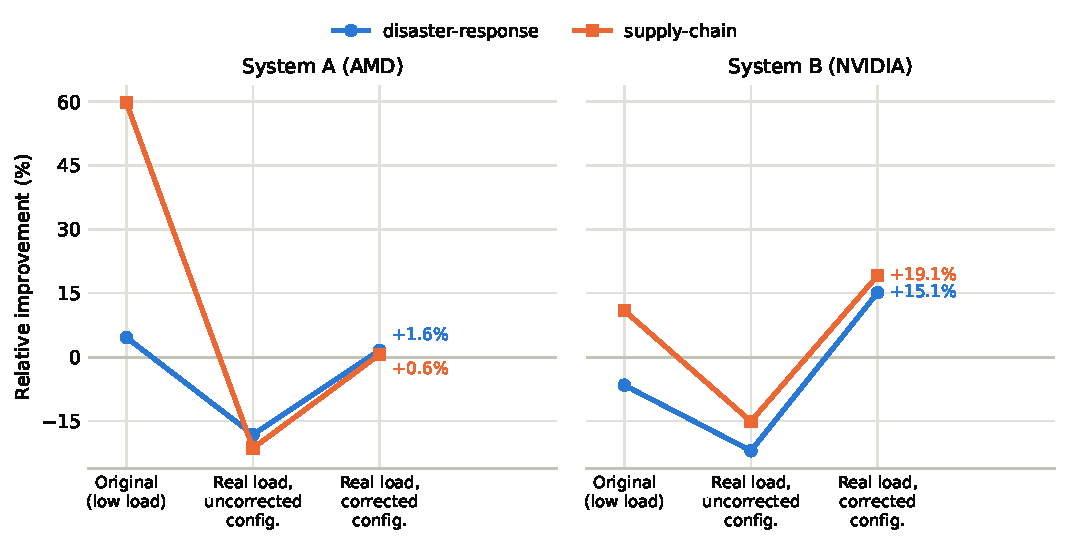
\includegraphics[width=\textwidth]{figures/fig_confound_b2.pdf}
\caption{Relative improvement of the platform-tuned configuration over common-denominator across the three investigation stages of Table~\ref{tab:b2-stages}, faceted by system. System A converges toward the zero baseline (a genuine tie); System B ends with a real, positive improvement on both workloads.}
\label{fig:confound-b2}
\end{figure}

Table~\ref{tab:b2-stages} and Figure~\ref{fig:confound-b2} summarize the three stages together. We found zero cache-eviction preemption across every one of these real runs, checked directly in server logs rather than by automated pattern matching alone, which confirms the effect is a batching and queueing efficiency phenomenon rather than the frozen procedure's hard disqualifier.

\subsection{The scheduling decision gate under real concurrent load}
\label{sec:scheduler-gate}

The scheduling-strategy decision gate (preregistered: at least 15\% relative improvement of the \Full{} strategy over \CausalOnly{}, non-overlapping, on heterogeneity-bearing workload variants) was first evaluated on a synthetic latency-simulating harness and, separately, on a real full-ladder pilot against live servers on both systems, both at an agent roster size of one replica per role. That real-hardware evidence showed \Full{} matching or exceeding every other strategy (System B: highest of all seven, $+80.2\%$ over \Sequential{}; System A: in line with \CausalOnly{}).

Given Section~\ref{sec:b2-confound}'s finding that this exact measurement regime (roster size, per-tick event cap, scheduling worker-pool cap) hid or inverted a real effect elsewhere, we reran the full ladder under the same real-load settings that reversed Section~\ref{sec:b2-confound}. \Full{} collapsed to a large, real regression, System B $-73.2\%$, System A $-71.6\%$, both non-overlapping, the opposite of the earlier conclusion.

Diagnosing this uncovered two further, independent, previously unknown confounds, neither related to roster size. First, four of the seven strategies (\Barrier{}, \CapabilityAware{}, \QueueAware{}, \Full{}) all defaulted to an internal per-round batching cap of 8 requests, independent of any worker-pool setting, forcing several sequential dispatch rounds per tick regardless of how large the worker pool was configured. Correcting this fully resolved \NaiveConcurrent{}, \Barrier{}, \CausalOnly{}, and \CapabilityAware{} into a tight, mutually indistinguishable cluster on both systems, previously roughly 3$\times$ apart. Second, \QueueAware{} and \Full{}'s per-provider in-flight concurrency cap, set at 4, had itself been tuned under the same insufficient-load regime, the exact structural parallel to Section~\ref{sec:b2-confound}'s serving-parameter bug. Even with the first confound fixed, \Full{} remained a large, real regression (System A $-66.1\%$, System B $-63.8\%$). A real sweep of the cap under genuine load found 4 a real, non-overlapping loser on both systems; 64 ties with 128 and wins the tie-break, closely matching \CausalOnly{}'s own throughput.

With both confounds corrected, a final confirmatory rerun found all six concurrent scheduling strategies statistically indistinguishable from one another on both systems (\Full{} versus \CausalOnly{}: System A $+1.1\%$, System B $-0.3\%$, both overlapping), with zero preemption and zero excluded repetitions across every real run in this investigation.

\begin{table}[t]
\centering
\small
\caption{Relative improvement of \Full{} over \CausalOnly{}, by stage of the investigation (Section~\ref{sec:scheduler-gate}). The ``original'' stage is reported qualitatively in our logs (overlapping bands) with no exact point estimate.}
\label{tab:scheduler-stages}
\begin{tabular}{lll}
\toprule
Stage & System A (AMD) & System B (NVIDIA) \\
\midrule
Low concurrency (original) & tied / \Full{} recovers & tied / \Full{} highest of 7 \\
Real load, uncorrected & $-71.6\%$ (real) & $-73.2\%$ (real) \\
Real load, batch-cap fixed & $-66.1\%$ (real) & $-63.8\%$ (real) \\
Real load, both fixed & $+1.1\%$ (overlap) & $-0.3\%$ (overlap) \\
\bottomrule
\end{tabular}
\end{table}

\begin{figure}[t]
\centering
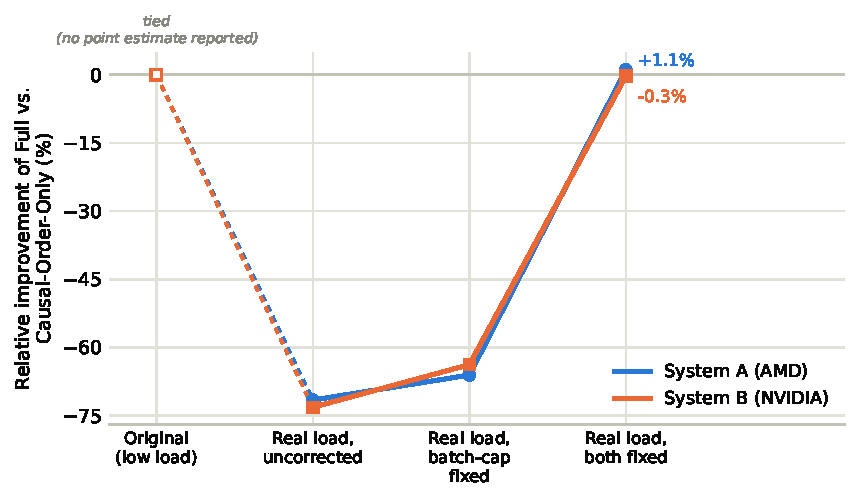
\includegraphics[width=0.78\textwidth]{figures/fig_confound_scheduler.pdf}
\caption{Relative improvement of \Full{} over \CausalOnly{} across the four investigation stages of Table~\ref{tab:scheduler-stages}. The hollow marker and dotted segment mark the first stage's qualitative ``tied'' result, for which no point estimate was reported; the three solid, measured stages show the collapse to a large regression and its full recovery once both confounds are corrected.}
\label{fig:confound-scheduler}
\end{figure}

Table~\ref{tab:scheduler-stages} and Figure~\ref{fig:confound-scheduler} summarize the four stages together. The decision gate is not cleared. We do not read this as evidence that capability-aware, queue-aware, or prefix-grouping scheduling is ineffective; we read it as evidence that the one workload class currently testable on real hardware provides no genuine multi-provider heterogeneity. Every real agent in every real run in this study routes to the same single serving endpoint, so the \CapabilityAware{} strategy's per-provider capability gate and the \QueueAware{} strategy's per-provider backpressure budget have nothing to differentiate. The mechanism has never been tested under the condition it is designed for, and Section~\ref{sec:limitations} discusses what that test requires.

\subsection{Cross-system portability}
\label{sec:portability}

The same simulation specification executes unmodified on both accelerator ecosystems, producing zero causal-verification violations and identical structural invariants on every real run reported above. All cross-system comparisons in this paper are within-system, normalized effect sizes (Section~\ref{sec:stats}); we do not report or interpret absolute cross-system throughput ratios as isolating accelerator-vendor effects (Section~\ref{sec:non-claims}).
